\documentclass[letterpaper]{article}
\usepackage[margin=1in]{geometry} % Sets page size and 1-inch margins
\usepackage[svgnames,dvipsnames]{xcolor}   % For a wider range of colors

\usepackage{amsmath} % For math symbols like \to, \langle, \rangle
\usepackage{array}   % For advanced column specifications
\usepackage{tabularx}% For tables with auto-expanding columns
\usepackage{tikz}
\usetikzlibrary{
    positioning,      % For placing nodes relative to each other (e.g., below=of)
    shapes.geometric, % For shapes like ellipses
    arrows.meta,      % For advanced arrow tips (e.g., Stealth)
    decorations.pathmorphing, % For snake/squiggly lines
    calc              % For coordinate calculations
}

% --- GLOBAL STYLE DEFINITIONS FOR DFD ---
\tikzset{
    % A shape for logical connectives
    connective_node/.style={
        rectangle, rounded corners=5pt, draw=black!80, fill=black!10,
        inner sep=5pt, thick, align=center
    },
    % A shape for Introduction Rules
    intro_rule_node/.style={
        rectangle, rounded corners=5pt, draw=black!80, fill=Teal!20,
        inner sep=5pt, thick, align=center
    },
    % A shape for Elimination Rules
    elim_rule_node/.style={
        rectangle, rounded corners=5pt, draw=black!80, fill=BurntOrange!20,
        inner sep=5pt, thick, align=center
    },
    % A shape for abstract propositions
    proposition_node/.style={
        ellipse, draw=black!80, fill=Violet!15,
        inner sep=3pt, align=center
    },
    % A shape for concrete proof terms
    proof_node/.style={
        ellipse, draw=black!80, fill=Green!15,
        inner sep=3pt, align=center
    },
    % Arrow styles with color
    input_arrow/.style={-Stealth, solid, thick, draw=blue!70!black},
    output_arrow/.style={double, double distance=1.5pt, -Stealth, solid, thick, draw=ForestGreen!80!black},
    proves_arrow/.style={-Stealth, decorate, decoration={snake, segment length=6pt, amplitude=1pt}, thick, draw=orange!90!black}
}

% --- Define and measure boxes to get widths for tabularx ---
\newlength{\impliesheaderwidth}
\settowidth{\impliesheaderwidth}{\textbf{Implies} : Prop $\to$ Prop $\to$ Prop}
\addtolength{\impliesheaderwidth}{1em}

\begin{document}

\begin{figure}[h!]
\centering
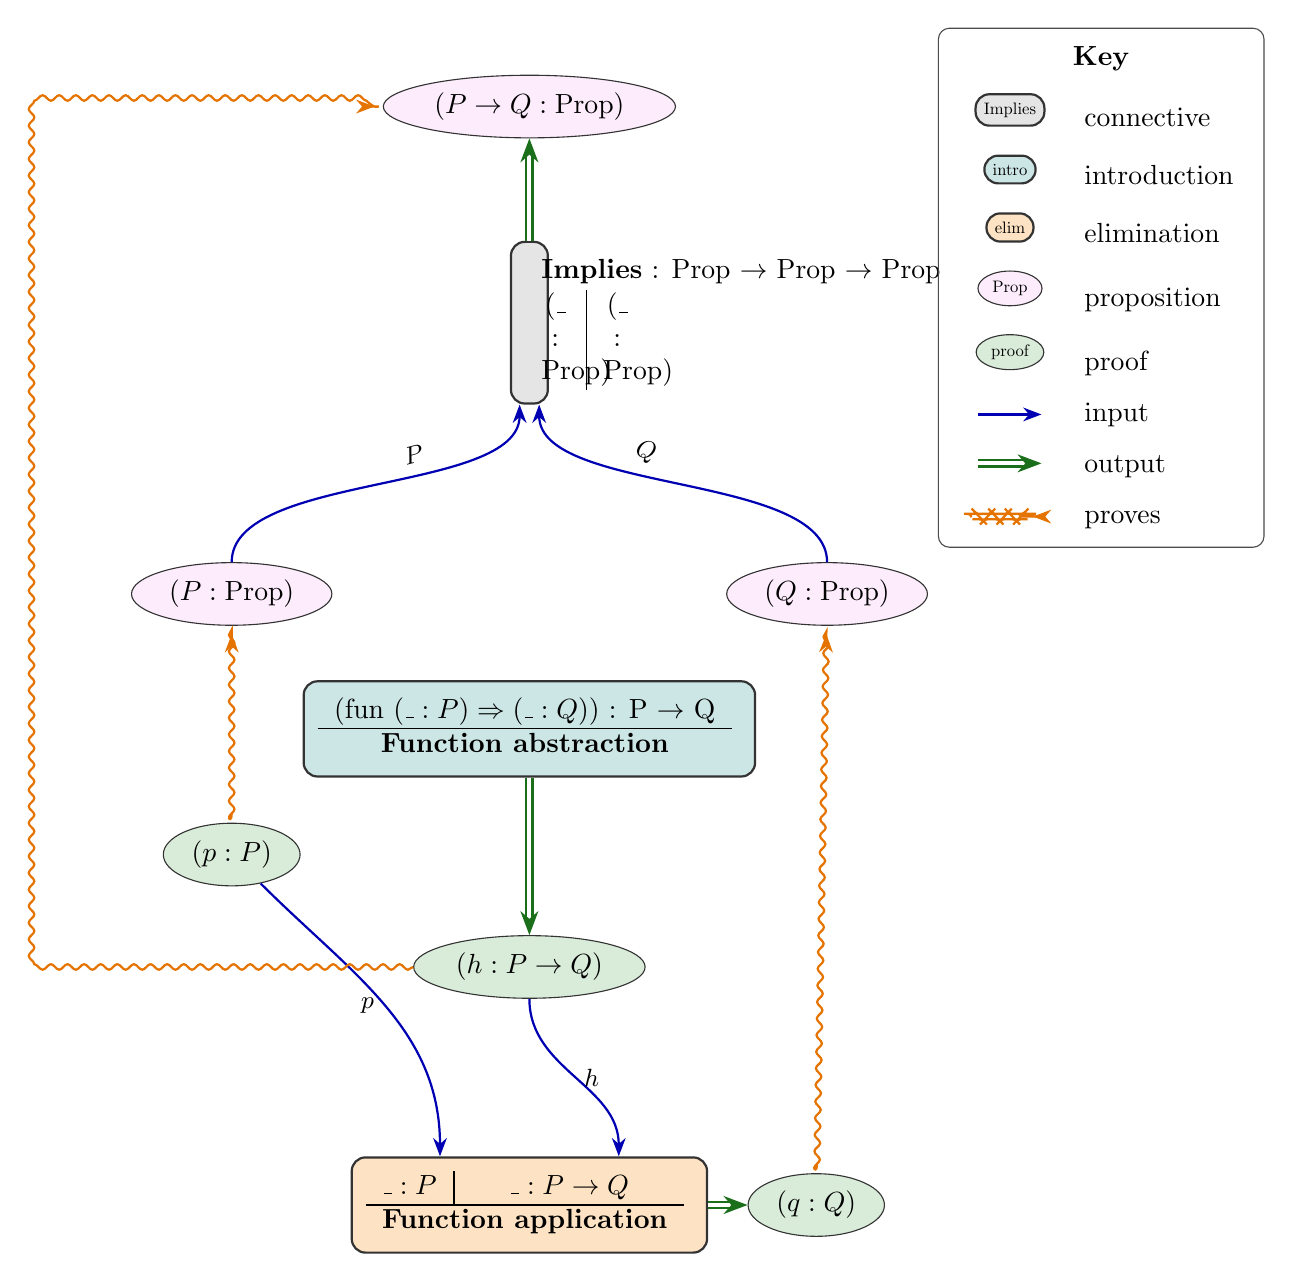
\begin{tikzpicture}[node distance=2cm and 2.5cm]

% --- OPTIMIZED NODE LAYOUT ---

% Top proposition layer - well spaced
\node[proposition_node] (P_prop) {$(P : \text{Prop})$};
\node[proposition_node] (Q_prop) [right=5cm of P_prop] {$(Q : \text{Prop})$};

% Connective layer
\node[connective_node, above=2cm of $(P_prop.north)!.5!(Q_prop.north)$] (implies_box) {
    \begin{tabularx}{\impliesheaderwidth}{>{\centering\arraybackslash}X|>{\centering\arraybackslash}X}
        \multicolumn{2}{c}{\textbf{Implies} : Prop $\to$ Prop $\to$ Prop} \\ \hline
        (\_ : Prop) & (\_ : Prop)
    \end{tabularx}
};

\node[proposition_node] (P_implies_Q_prop) [above=1.3cm of implies_box] {$(P \to Q : \text{Prop})$};

% Introduction layer - centered and clean
\node[intro_rule_node, below=1.5cm of $(P_prop.north)!.5!(Q_prop.north)$] (implies_intro) {
    \begin{tabular}{c}
    $(\text{fun } (\_ : P) \Rightarrow (\_ : Q))$ : P $\to$ Q \\ \hline
    \textbf{Function abstraction}
    \end{tabular}
};

\node[proof_node] (f_P_to_Q) [below=2cm of implies_intro] {$(h : P \to Q)$};

% Proof layer - symmetrically positioned
\node[proof_node] (p_premise) [below=2.5cm of P_prop] {$(p : P)$};

% Elimination layer - optimally positioned
\node[elim_rule_node, below=2cm of f_P_to_Q] (implies_elim) {
    \begin{tabular}{c|c}
    $\_ : P$ & $\_ : P \to Q$ \\ \hline
    \multicolumn{2}{c}{\textbf{Function application}}
    \end{tabular}
};

\node[proof_node] (result_Q) [right=0.5cm of implies_elim] {$(q : Q)$};

% --- OPTIMIZED EDGE ROUTING ---

% Top level connections
\draw[output_arrow] (implies_box) -> (P_implies_Q_prop);
\draw[input_arrow] (P_prop.north) to[out=90, in=-90, looseness=0.7] node[pos=0.6, sloped, above, font=\small] {$P$} ($(implies_box.south west)!.5!(implies_box.south)$);
\draw[input_arrow] (Q_prop.north) to[out=90, in=-90, looseness=0.7] node[pos=0.6, sloped, above, font=\small] {$Q$} ($(implies_box.south)!.5!(implies_box.south east)$);

% Introduction flow
\draw[output_arrow] (implies_intro) -> (f_P_to_Q);

% Elimination flow - arrows to middle of cells
\draw[input_arrow] (p_premise) to[out=-45, in=90] node[pos=0.5, left, font=\small] {$p$} ($(implies_elim.north west)!.5!(implies_elim.north)$);
\draw[input_arrow] (f_P_to_Q) to[out=-90, in=90] node[pos=0.5, right, font=\small] {$h$} ($(implies_elim.north)!.5!(implies_elim.north east)$);

% Output from elimination
\draw[output_arrow] (implies_elim.east) -> (result_Q.west);



% Type/proves arrows - clean and direct
\draw[proves_arrow, shorten <=3pt, shorten >=3pt] (p_premise) -> (P_prop);
\draw[proves_arrow, shorten <=3pt, shorten >=3pt] (result_Q) -> (Q_prop);

% Main "proves" arc for the constructed function
\coordinate (outset_point) at ($(P_prop.west)+(-1.2cm,0)$);
\draw[proves_arrow, shorten >=3pt] (f_P_to_Q.west) -- (outset_point |- f_P_to_Q.west) -- (outset_point |- P_implies_Q_prop.west) -- (P_implies_Q_prop.west);

% --- LEGEND ---
\node (legend) [draw=black!70, rounded corners, inner sep=5pt, above right=0.3cm and 0.5cm of Q_prop] {
    \begin{tabular}{cl}
    \multicolumn{2}{c}{\textbf{Key}} \\[1.5ex]
    \tikz{\node[connective_node, scale=0.6] {Implies};} & connective \\[1.5ex]
    \tikz{\node[intro_rule_node, scale=0.6] {intro};} & introduction \\[1.5ex]
    \tikz{\node[elim_rule_node, scale=0.6] {elim};} & elimination \\[1.5ex]
    \tikz{\node[proposition_node, scale=0.6] {Prop};} & proposition \\[1.5ex]
    \tikz{\node[proof_node, scale=0.6] {proof};} & proof \\[1.5ex]
    \tikz{\draw[input_arrow] (0,0.1) -- (0.8,0.1);} & input \\[1.5ex]
    \tikz{\draw[output_arrow] (0,0.1) -- (0.8,0.1);} & output \\[1.5ex]
    \tikz{\draw[proves_arrow] (0,0.1) -- (0.8,0.1);} & proves \\
    \end{tabular}
};

\end{tikzpicture}
\caption{The algebra of logical implication. The Implies function builds the proposition
$P \to Q$ from two propositions $P$ and $Q$. In constructive logic, implication is 
realized as the function type constructor: a proof of $P \to Q$ is literally a function 
that transforms proofs of $P$ into proofs of $Q$. The introduction rule uses function 
abstraction: to prove $P \to Q$, assume $P$ as a hypothesis and derive $Q$, then 
abstract over the assumption using lambda (written as \texttt{fun} in Lean). The 
elimination rule is function application (modus ponens): given a proof $h : P \to Q$ 
and a proof $p : P$, applying $h$ to $p$ yields a proof of $Q$. This direct 
correspondence between logical implication and functional programming embodies the 
Curry-Howard isomorphism at its most fundamental level.}\label{fig:tikz_diagram_implies}
\end{figure}

\end{document}